% Options for packages loaded elsewhere
\PassOptionsToPackage{unicode}{hyperref}
\PassOptionsToPackage{hyphens}{url}
%
\documentclass[
]{book}
\usepackage{amsmath,amssymb}
\usepackage{lmodern}
\usepackage{iftex}
\ifPDFTeX
  \usepackage[T1]{fontenc}
  \usepackage[utf8]{inputenc}
  \usepackage{textcomp} % provide euro and other symbols
\else % if luatex or xetex
  \usepackage{unicode-math}
  \defaultfontfeatures{Scale=MatchLowercase}
  \defaultfontfeatures[\rmfamily]{Ligatures=TeX,Scale=1}
\fi
% Use upquote if available, for straight quotes in verbatim environments
\IfFileExists{upquote.sty}{\usepackage{upquote}}{}
\IfFileExists{microtype.sty}{% use microtype if available
  \usepackage[]{microtype}
  \UseMicrotypeSet[protrusion]{basicmath} % disable protrusion for tt fonts
}{}
\makeatletter
\@ifundefined{KOMAClassName}{% if non-KOMA class
  \IfFileExists{parskip.sty}{%
    \usepackage{parskip}
  }{% else
    \setlength{\parindent}{0pt}
    \setlength{\parskip}{6pt plus 2pt minus 1pt}}
}{% if KOMA class
  \KOMAoptions{parskip=half}}
\makeatother
\usepackage{xcolor}
\IfFileExists{xurl.sty}{\usepackage{xurl}}{} % add URL line breaks if available
\IfFileExists{bookmark.sty}{\usepackage{bookmark}}{\usepackage{hyperref}}
\hypersetup{
  pdftitle={My portfolio},
  pdfauthor={Claudia van der Zijden},
  hidelinks,
  pdfcreator={LaTeX via pandoc}}
\urlstyle{same} % disable monospaced font for URLs
\usepackage{color}
\usepackage{fancyvrb}
\newcommand{\VerbBar}{|}
\newcommand{\VERB}{\Verb[commandchars=\\\{\}]}
\DefineVerbatimEnvironment{Highlighting}{Verbatim}{commandchars=\\\{\}}
% Add ',fontsize=\small' for more characters per line
\usepackage{framed}
\definecolor{shadecolor}{RGB}{248,248,248}
\newenvironment{Shaded}{\begin{snugshade}}{\end{snugshade}}
\newcommand{\AlertTok}[1]{\textcolor[rgb]{0.94,0.16,0.16}{#1}}
\newcommand{\AnnotationTok}[1]{\textcolor[rgb]{0.56,0.35,0.01}{\textbf{\textit{#1}}}}
\newcommand{\AttributeTok}[1]{\textcolor[rgb]{0.77,0.63,0.00}{#1}}
\newcommand{\BaseNTok}[1]{\textcolor[rgb]{0.00,0.00,0.81}{#1}}
\newcommand{\BuiltInTok}[1]{#1}
\newcommand{\CharTok}[1]{\textcolor[rgb]{0.31,0.60,0.02}{#1}}
\newcommand{\CommentTok}[1]{\textcolor[rgb]{0.56,0.35,0.01}{\textit{#1}}}
\newcommand{\CommentVarTok}[1]{\textcolor[rgb]{0.56,0.35,0.01}{\textbf{\textit{#1}}}}
\newcommand{\ConstantTok}[1]{\textcolor[rgb]{0.00,0.00,0.00}{#1}}
\newcommand{\ControlFlowTok}[1]{\textcolor[rgb]{0.13,0.29,0.53}{\textbf{#1}}}
\newcommand{\DataTypeTok}[1]{\textcolor[rgb]{0.13,0.29,0.53}{#1}}
\newcommand{\DecValTok}[1]{\textcolor[rgb]{0.00,0.00,0.81}{#1}}
\newcommand{\DocumentationTok}[1]{\textcolor[rgb]{0.56,0.35,0.01}{\textbf{\textit{#1}}}}
\newcommand{\ErrorTok}[1]{\textcolor[rgb]{0.64,0.00,0.00}{\textbf{#1}}}
\newcommand{\ExtensionTok}[1]{#1}
\newcommand{\FloatTok}[1]{\textcolor[rgb]{0.00,0.00,0.81}{#1}}
\newcommand{\FunctionTok}[1]{\textcolor[rgb]{0.00,0.00,0.00}{#1}}
\newcommand{\ImportTok}[1]{#1}
\newcommand{\InformationTok}[1]{\textcolor[rgb]{0.56,0.35,0.01}{\textbf{\textit{#1}}}}
\newcommand{\KeywordTok}[1]{\textcolor[rgb]{0.13,0.29,0.53}{\textbf{#1}}}
\newcommand{\NormalTok}[1]{#1}
\newcommand{\OperatorTok}[1]{\textcolor[rgb]{0.81,0.36,0.00}{\textbf{#1}}}
\newcommand{\OtherTok}[1]{\textcolor[rgb]{0.56,0.35,0.01}{#1}}
\newcommand{\PreprocessorTok}[1]{\textcolor[rgb]{0.56,0.35,0.01}{\textit{#1}}}
\newcommand{\RegionMarkerTok}[1]{#1}
\newcommand{\SpecialCharTok}[1]{\textcolor[rgb]{0.00,0.00,0.00}{#1}}
\newcommand{\SpecialStringTok}[1]{\textcolor[rgb]{0.31,0.60,0.02}{#1}}
\newcommand{\StringTok}[1]{\textcolor[rgb]{0.31,0.60,0.02}{#1}}
\newcommand{\VariableTok}[1]{\textcolor[rgb]{0.00,0.00,0.00}{#1}}
\newcommand{\VerbatimStringTok}[1]{\textcolor[rgb]{0.31,0.60,0.02}{#1}}
\newcommand{\WarningTok}[1]{\textcolor[rgb]{0.56,0.35,0.01}{\textbf{\textit{#1}}}}
\usepackage{longtable,booktabs,array}
\usepackage{calc} % for calculating minipage widths
% Correct order of tables after \paragraph or \subparagraph
\usepackage{etoolbox}
\makeatletter
\patchcmd\longtable{\par}{\if@noskipsec\mbox{}\fi\par}{}{}
\makeatother
% Allow footnotes in longtable head/foot
\IfFileExists{footnotehyper.sty}{\usepackage{footnotehyper}}{\usepackage{footnote}}
\makesavenoteenv{longtable}
\usepackage{graphicx}
\makeatletter
\def\maxwidth{\ifdim\Gin@nat@width>\linewidth\linewidth\else\Gin@nat@width\fi}
\def\maxheight{\ifdim\Gin@nat@height>\textheight\textheight\else\Gin@nat@height\fi}
\makeatother
% Scale images if necessary, so that they will not overflow the page
% margins by default, and it is still possible to overwrite the defaults
% using explicit options in \includegraphics[width, height, ...]{}
\setkeys{Gin}{width=\maxwidth,height=\maxheight,keepaspectratio}
% Set default figure placement to htbp
\makeatletter
\def\fps@figure{htbp}
\makeatother
\setlength{\emergencystretch}{3em} % prevent overfull lines
\providecommand{\tightlist}{%
  \setlength{\itemsep}{0pt}\setlength{\parskip}{0pt}}
\setcounter{secnumdepth}{5}
\usepackage{booktabs}
\ifLuaTeX
  \usepackage{selnolig}  % disable illegal ligatures
\fi
\usepackage[]{natbib}
\bibliographystyle{apalike}

\title{My portfolio}
\author{Claudia van der Zijden}
\date{2021-06-20}

\begin{document}
\maketitle

{
\setcounter{tocdepth}{1}
\tableofcontents
}
\hypertarget{introduction}{%
\chapter{Introduction}\label{introduction}}

Welkom to my portfolio!

In my portfolio I try to give an impression of my programming skills. This is mainly in r but I also have some experience with bash.

This portfolio contains a number of chapters with assignments that I have made, it also contains my resume. The last chapter called machine learning is about a tutorial assignment in which I tried to learn more about machine learning.

I hope this portfolio will give you a good idea of my skills.

For further questions you can always email \href{mailto:claudiavanderzijden@hotmail.nl}{\nolinkurl{claudiavanderzijden@hotmail.nl}}

\hypertarget{reproducible-research}{%
\chapter{Reproducible research}\label{reproducible-research}}

C. elegans plate experiment

\emph{The data for this exercise was kindly supplied by J. Louter (INT/ILC) and was derived from an experiment in which adult C.elegans nematodes were exposed to varying concentrations of different compounds. The variables RawData (the outcome - number of offspring counted as an integer value, after incubation time), compName (the generic name of the compound/chemical), the compConcentration (the concentration of the compound), and the expType are the most important variables in this dataset.}

\emph{A typical analysis with this data would be to run a dose-response analysis using a log-logistic model with estimates for the maximal, the minimal, the IC50 concentration and the slope at IC50. We will not go into the details but a good package to run such computations and create graphs in R is the \{drc\} package. See: and:. In the exercise below we will create some visualizations using \{ggplot2\}.}

Before we start, we will inspect the dataset. We do this by opening it in Excel. When you look at this dataset, a few things stand out. Among other things, there are many tabs with very large tables without an explanation. This makes it difficult for outsiders to use this data.

Then we will load the data into rstudio.

\begin{Shaded}
\begin{Highlighting}[]
\FunctionTok{library}\NormalTok{(tidyverse)}
\end{Highlighting}
\end{Shaded}

\begin{verbatim}
## -- Attaching packages --------------------------------------- tidyverse 1.3.1 --
\end{verbatim}

\begin{verbatim}
## v ggplot2 3.3.3     v purrr   0.3.4
## v tibble  3.1.2     v dplyr   1.0.6
## v tidyr   1.1.3     v stringr 1.4.0
## v readr   1.4.0     v forcats 0.5.1
\end{verbatim}

\begin{verbatim}
## -- Conflicts ------------------------------------------ tidyverse_conflicts() --
## x dplyr::filter() masks stats::filter()
## x dplyr::lag()    masks stats::lag()
\end{verbatim}

\begin{Shaded}
\begin{Highlighting}[]
\FunctionTok{library}\NormalTok{(readxl)}
\NormalTok{ce\_liq\_flow\_062 }\OtherTok{\textless{}{-}} \FunctionTok{read\_excel}\NormalTok{(}\StringTok{"data/CE.LIQ.FLOW.062\_Tidydata.xlsx"}\NormalTok{, }\AttributeTok{sheet =} \DecValTok{1}\NormalTok{)}
\end{Highlighting}
\end{Shaded}

Now we can look at the data types. we will do this for the columns rawData, compName and compConcentration.

\begin{Shaded}
\begin{Highlighting}[]
\FunctionTok{typeof}\NormalTok{(ce\_liq\_flow\_062}\SpecialCharTok{$}\NormalTok{RawData)}
\end{Highlighting}
\end{Shaded}

\begin{verbatim}
## [1] "double"
\end{verbatim}

\begin{Shaded}
\begin{Highlighting}[]
\FunctionTok{typeof}\NormalTok{(ce\_liq\_flow\_062}\SpecialCharTok{$}\NormalTok{compName)}
\end{Highlighting}
\end{Shaded}

\begin{verbatim}
## [1] "character"
\end{verbatim}

\begin{Shaded}
\begin{Highlighting}[]
\FunctionTok{typeof}\NormalTok{(ce\_liq\_flow\_062}\SpecialCharTok{$}\NormalTok{compConcentration)}
\end{Highlighting}
\end{Shaded}

\begin{verbatim}
## [1] "character"
\end{verbatim}

You would expect comConcentration to be numeric but as you can see this is character.

Now we are going to make a scatter plot of the data. We put compconcentration on the x-axis and DataRaw on the y-axis. We give a different color to the levels of compname and a different shape to the levels of expType. In addition, we ensure that the numbers below the x-axis are rotated 45 degrees so that we can read those.

\begin{Shaded}
\begin{Highlighting}[]
\FunctionTok{ggplot}\NormalTok{(}\AttributeTok{data =}\NormalTok{ ce\_liq\_flow\_062, }\FunctionTok{aes}\NormalTok{(}\AttributeTok{x =}\NormalTok{ compConcentration, }\AttributeTok{y =}\NormalTok{ RawData)) }\SpecialCharTok{+}
  \FunctionTok{geom\_point}\NormalTok{(}\FunctionTok{aes}\NormalTok{(}\AttributeTok{colour =}\NormalTok{ compName, }\AttributeTok{shape =}\NormalTok{ expType)) }\SpecialCharTok{+}
   \FunctionTok{scale\_x\_discrete}\NormalTok{(}\AttributeTok{guide =} \FunctionTok{guide\_axis}\NormalTok{(}\AttributeTok{angle =} \DecValTok{45}\NormalTok{)) }\SpecialCharTok{+}
  \FunctionTok{labs}\NormalTok{(}\AttributeTok{title =} \StringTok{"compConcentration is double"}\NormalTok{)}
\end{Highlighting}
\end{Shaded}

\begin{verbatim}
## Warning: Removed 5 rows containing missing values (geom_point).
\end{verbatim}

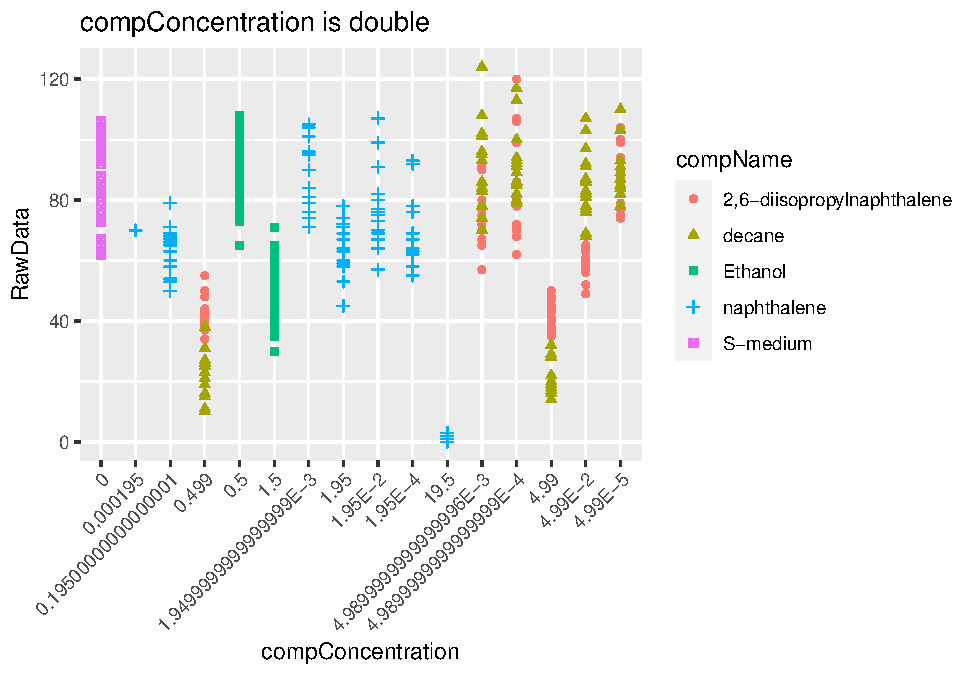
\includegraphics{Nexttry_files/figure-latex/1.1D-1.pdf}

If we now look at this plot, you can see that the scale of the x-axis is not linearly distributed. This is probably due to the data type of comcondition. So we're going to change it to numeric. Then we will plot the data again. We now use a log10 transformation to improve the distribution of the x-axis. We also use jitter to avoid overlapping data points.

\begin{Shaded}
\begin{Highlighting}[]
\NormalTok{ce\_liq\_flow\_062}\SpecialCharTok{$}\NormalTok{compConcentration }\OtherTok{\textless{}{-}} \FunctionTok{as.numeric}\NormalTok{(}\FunctionTok{as.character}\NormalTok{(ce\_liq\_flow\_062}\SpecialCharTok{$}\NormalTok{compConcentration))}
\end{Highlighting}
\end{Shaded}

\begin{verbatim}
## Warning: NAs introduced by coercion
\end{verbatim}

\begin{Shaded}
\begin{Highlighting}[]
\FunctionTok{typeof}\NormalTok{(ce\_liq\_flow\_062}\SpecialCharTok{$}\NormalTok{compConcentration)}
\end{Highlighting}
\end{Shaded}

\begin{verbatim}
## [1] "double"
\end{verbatim}

\begin{Shaded}
\begin{Highlighting}[]
\NormalTok{log10\_scatter }\OtherTok{\textless{}{-}}\FunctionTok{ggplot}\NormalTok{(}\AttributeTok{data =}\NormalTok{ ce\_liq\_flow\_062, }\FunctionTok{aes}\NormalTok{(}\AttributeTok{x =}\NormalTok{ compConcentration, }\AttributeTok{y =}\NormalTok{ RawData)) }\SpecialCharTok{+}
  \FunctionTok{geom\_point}\NormalTok{(}\AttributeTok{position=}\FunctionTok{position\_jitter}\NormalTok{(}\AttributeTok{width=}\NormalTok{.}\DecValTok{1}\NormalTok{,}\AttributeTok{height=}\DecValTok{0}\NormalTok{),}\FunctionTok{aes}\NormalTok{(}\AttributeTok{colour =}\NormalTok{ compName, }\AttributeTok{shape =}\NormalTok{ compName)) }\SpecialCharTok{+}
   \FunctionTok{scale\_x\_discrete}\NormalTok{(}\AttributeTok{guide =} \FunctionTok{guide\_axis}\NormalTok{(}\AttributeTok{angle =} \DecValTok{45}\NormalTok{))}\SpecialCharTok{+}
   \FunctionTok{labs}\NormalTok{(}\AttributeTok{title =} \StringTok{"compConcentration is numeric"}\NormalTok{) }


\NormalTok{log10\_scatter }\SpecialCharTok{+} \FunctionTok{scale\_x\_log10}\NormalTok{()}
\end{Highlighting}
\end{Shaded}

\begin{verbatim}
## Scale for 'x' is already present. Adding another scale for 'x', which will
## replace the existing scale.
\end{verbatim}

\begin{verbatim}
## Warning: Transformation introduced infinite values in continuous x-axis
\end{verbatim}

\begin{verbatim}
## Warning: Removed 6 rows containing missing values (geom_point).
\end{verbatim}

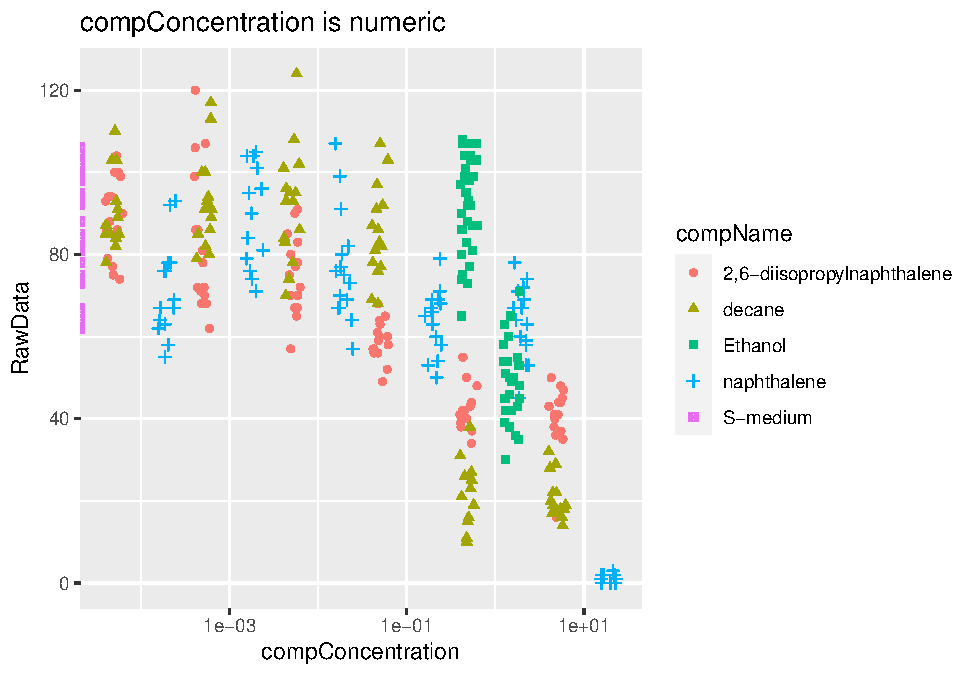
\includegraphics{Nexttry_files/figure-latex/1.1F-1.pdf}

The positive control for this experiments is \textbf{naphthale}. The negative control for this experiment is \textbf{S-medium}.

After reviewing the data, we could proceed with the analysis of the data to find out whether there is indeed an effect of different concentrations on offspring count and whether the different compounds have a different curve. To find out, first check whether the data is normally distributed. This can be done with the shapio-wilk test. This can be used to determine whether a parametric or non-parametric test can be used to see if there is a statistically significant difference between the different groups.

Finaly we normalize the data for the controlNegative in such a way that the mean value for controlNegative is exactly equal to 1 and all other values are expressed as a fraction thereof. Than we rerun the graph with the normalized data.

\#``\{r 1.1J\}
normalize \textless- function(x) \{
return ((x - min(x)) / (max(x) - min(x)))
\}

ce\_liq\_flow\_062\(compVehicle %>% normalize(filter(ce_liq_flow_062
\)compVehicle == ``controlNegative''))

\begin{verbatim}


H.Why would you want to take the step under J?

<!--chapter:end:01-Reproducible_Research.Rmd-->

# Open Peer Review

In this assisgment w arw goning to find a scientific article ourself, using PubMed or another database or repository. We'll use only Open Access articles. When we fond a article we will go over the Transparency Criteria.

This is the link to the article I use
https://www.biorxiv.org/content/10.1101/2020.10.02.322917v2.full

The title of this article is: Leveraging high-throughput screening data and conditional generative adversarial networks to advance predictive toxicology
The authors of this article are: Adrian J. Green, Martin J. Mohlenkamp, Jhuma Das, et al.

## Peer revieuw part 1

__Study Purpose__ : the summary briefly explains what is more important to conduct this research <br/>
__Data Availability Statement__: not present <br/>
__Data Location__: it does describe what the data should look like and there are references to articles that describe how the data was collected. It does not say where you can find the used data. <br/>
__Study Location__: there is no information about where the study was conducted in the material and method section <br/>
__Author Review__: the details of the authors are not easy to obtain, the names of the authors are at the top of the article but further contact details are not on the page itself. <br/>
__Ethics Statement__: the introduction briefly mentions ethics <br/>
__Funding Statement__: nothing is said about funding <br/>
__Code Availability__: no code is shared in the article <br/>

## Open peer review part 2
Next we are going to try to find a article with R code. We do this on the OSF website.
We are going to try to get the code working in our r studio. 

This is the link to the code we will use
https://osf.io/gkcn7/

To make this code work we only have to change the way to load the data, out commend the effect sizes and we have to change the column names so the names are not separated by points. 

You can find the working script in the appendix, chapther 11

It took little effort to get this script working. On a scale of 0 to 5 I would give it a 4

<!--chapter:end:02-Open_peer_review.Rmd-->

# Guerrilla analytics

In this assignment I cleaned up my projects according to the Guerrilla analytics.The result can be seen below onder. 

## Daur2 project
![Claudia](data/Gurilla/Daur2.png){ width=70%}


## Portfolio project
![Claudia](data/Gurilla/portfolio.png){ width=70%}


## Project project
![Claudia](data/Gurilla/project.png){ width=70%}





<!--chapter:end:03-Guerrilla_analytics.Rmd-->

# Curriculum vitae

![Claudia](data/CV/cvfoto.png){ width=100%}

<!--chapter:end:04-Curriculum_vitae.Rmd-->

# Mendaly

In practice, many use has been made of RNA sequencing (RNA-seq) methods. With RNA-seq, the transcriptional activity of cells can be examined. Next-generation sequencing is used for this. This results in transcriptomics datasets, which makes it difficult for many researchers to process this data and to draw conclusions from it. [@Marini2020]. That is why in this project we are working on a way in which researchers without programming knowledge can easily process transcriptome data. The aim is to develop a shiny app where only a GSE/SRA number needs to be entered, after which an analysis is performed automatically. This saves researchers a lot of time. To make this possible, we use salmon and DESeq2 among others. A GSE number can be used to search the SRA database for a dataset in the form of a fastq file. This fastq file can be used in Salmon. Salmon is a package that quantifies the data.[@Patro2017] . When quantifying the data, it is determined how many of the parts of the data correspond to the reference data. Because Salmon takes small pieces of the data for testing, it works much faster and takes much less memory to perform this analysis than other methods. The analyzed data that then comes from the salmon analysis will be further investigated using deseq2. The DESeq2 package provides methods to test for differential expression using negative binomial generalized linear models. [@rnaseq] A sumerised experiment is then made of this data. [@sumexp] A sumerised experiment is a container where data is stored in different dimensions. It contains row data, it contains information about the genes, and the cold data also contains information about the samples. Finally, the sumerised experiment also contains the number of counts. A sumerised experiment will serve as input for the ISEE shiny app. This ISEE app has been specially developed for analyzing transcriptome data [@Lun2018] In this app not only the count data are processed, but also the row data and the cold data are displayed in graphs. This makes the analysis very comprehensive.
In our project we also want to pay attention to a new shiny app. Although the ISEE app is a well-functioning app, there are a number of things that we miss. For example, we think that the app is not clear enough because all graphs are plotted on one page without further additions. In addition, we miss a way in which you can enter the GSE/SRA number. So you still need some programming skills to use this app.
Ultimately, it would be nice if you only had to fill in a dataset and you would then receive a message as soon as the analysis is ready. At the moment this analysis is ready, it would be nice if a ready-made report could be downloaded with the result processing and statistical tests in it.

<!--chapter:end:05-Mendely.Rmd-->

# Relational databases

TIPS

Be aware, the flu and dengue data contains metadata that should be stripped from the data on load.
Think of a way to create valid country names that fit with the gapminder data.
Remember (!) that in the end, this assignment needs to be reported by a .Rmd file for your portfolio. So save what you are doing, save your SQL scripts, make screenshots if you want, and in general design a clear and attractive report in RMarkdown to showcase your SQL/database-skills in your portfolio. You may be sending this to propspective employers in the future! (also, the portfolio is what we as teachers will be grading. But definitely think about the future rather than only about “passing the course”)
Assignment

Load the flu (“./data/flu_data.csv), the dengue (.”/data/dengue_data.csv) and the gapminder ({dslabs} package) into three separate dataframes in R

Check if they are in the right shape. Is the data in the ‘tidy’ format? If not change the format to ‘tidy’

Change the country and date variables of the three tables so that they coincide in terms of data type, class and values

Store the three tables as separate (so six in total) .csv and .rds files.

In Dbeaver create a new PostgreSQL database “workflowsdb”

Using RPostgreSQL, insert the tables into the database.

Inspect the contents of the tables with SQL (in DBeaver) and save the SQL script.

Inspect the contents of the tables with dplyr (in R) and save a RMarkdown showing what you are doing.

Load the gapminder data in R and change the dataframe in such as way that you could join it to dengue and flue.

Save this clean gapminder data in the “workflowsdb” database

Perform some joins (your choice) with SQL (can be done in DBeaver or with dplyr.

Generate a joined table, and export this from the database to R.

Show some descriptive statistics with this table, and at least 3 visualisations using ggplot2.

show all of your actions in this assignment in a Rmd file, perhaps with pictures and provide text explaining and showcasing your skills.

```r
library(tidyverse)
library(dslabs)
gapminder <- as_tibble(gapminder)
flu_data<- read.csv(url("https://raw.githubusercontent.com/ClaudiavdZ/tlsc-dsfb26v-20_workflows/main/data/flu_data.csv"), skip = 11)
flu_data <- as_tibble(flu_data)
dengue_data<- read.csv(url("https://raw.githubusercontent.com/ClaudiavdZ/tlsc-dsfb26v-20_workflows/main/data/dengue_data.csv"), skip = 11)

write.table(dengue_data , file = "dengu_data.csv")
write.table(dengue_data , file = "dengu_data.RDS")
write.table(flu_data , file = "flu_data.csv")
write.table(flu_data , file = "flu_data.RDS")
write.table(gapminder , file = "gapminder.csv")
write.table(gapminder , file = "gapminder.RDS")

library(DBI)
con <- dbConnect(RPostgres::Postgres(), 
                 dbname = "myfirstdb", 
                 host="localhost", 
                 port="5432", 
                 user="postgres", 
                 password="Veroni36") 
dbListTables(con) 
\end{verbatim}

\begin{verbatim}
## [1] "test"        "gapminder"   "flu_data"    "dengue_data"
\end{verbatim}

\begin{Shaded}
\begin{Highlighting}[]
\CommentTok{\#dbWriteTable(con, "dengue\_data", dengue\_data)}
\CommentTok{\#dbWriteTable(con, "flu\_data", flu\_data)}
\CommentTok{\#dbWriteTable(con, "gapminder", gapminder)}

\CommentTok{\# library(janitor)}
\CommentTok{\# gapminder\_usd \textless{}{-} as.data.frame(t(gapminder))}
\CommentTok{\# gapminder\_usd \textless{}{-} gapminder\_usd \%\textgreater{}\% row\_to\_names(row\_number = 1)}


\NormalTok{flu\_usd }\OtherTok{\textless{}{-}} \FunctionTok{gather}\NormalTok{(}
\NormalTok{  flu\_data,}
  \AttributeTok{key =} \StringTok{"country"}\NormalTok{,}
  \AttributeTok{value =} \StringTok{"flu"}\NormalTok{,}
\NormalTok{  Argentina}\SpecialCharTok{:}\NormalTok{Uruguay}
\NormalTok{)}
\CommentTok{\#seperate year from month and day}
\NormalTok{flu\_usd }\OtherTok{\textless{}{-}} \FunctionTok{separate}\NormalTok{(flu\_usd, Date, }\AttributeTok{into =} \FunctionTok{c}\NormalTok{(}\StringTok{"year"}\NormalTok{, }\StringTok{"month"}\NormalTok{, }\StringTok{"day"}\NormalTok{),  }\AttributeTok{sep =} \StringTok{"{-}"}\NormalTok{)}
\CommentTok{\#count sum of flu}
\NormalTok{flu\_usd }\OtherTok{\textless{}{-}} \FunctionTok{aggregate}\NormalTok{(flu\_usd}\SpecialCharTok{$}\NormalTok{flu, }\AttributeTok{by=}\FunctionTok{list}\NormalTok{(}\AttributeTok{year=}\NormalTok{flu\_usd}\SpecialCharTok{$}\NormalTok{year, }\AttributeTok{country=}\NormalTok{flu\_usd}\SpecialCharTok{$}\NormalTok{country), }\AttributeTok{FUN=}\NormalTok{sum)}
\NormalTok{flu\_usd }\OtherTok{\textless{}{-}}\NormalTok{ flu\_usd }\SpecialCharTok{\%\textgreater{}\%} \FunctionTok{rename}\NormalTok{(}\AttributeTok{flu =}\NormalTok{ x)}
\NormalTok{flu\_usd}\SpecialCharTok{$}\NormalTok{year }\OtherTok{\textless{}{-}} \FunctionTok{as.integer}\NormalTok{(flu\_usd}\SpecialCharTok{$}\NormalTok{year)  }

\NormalTok{dengue\_usd }\OtherTok{\textless{}{-}} \FunctionTok{gather}\NormalTok{(}
\NormalTok{  dengue\_data,}
  \AttributeTok{key =} \StringTok{"country"}\NormalTok{,}
  \AttributeTok{value =} \StringTok{"dengue"}\NormalTok{,}
\NormalTok{  Argentina}\SpecialCharTok{:}\NormalTok{Venezuela}
\NormalTok{)}
\NormalTok{dengue\_usd }\OtherTok{\textless{}{-}} \FunctionTok{separate}\NormalTok{(dengue\_usd, Date, }\AttributeTok{into =} \FunctionTok{c}\NormalTok{(}\StringTok{"year"}\NormalTok{, }\StringTok{"month"}\NormalTok{, }\StringTok{"day"}\NormalTok{),  }\AttributeTok{sep =} \StringTok{"{-}"}\NormalTok{)}
\NormalTok{dengue\_usd }\OtherTok{\textless{}{-}} \FunctionTok{aggregate}\NormalTok{(dengue\_usd}\SpecialCharTok{$}\NormalTok{dengue, }\AttributeTok{by=}\FunctionTok{list}\NormalTok{(}\AttributeTok{year=}\NormalTok{dengue\_usd}\SpecialCharTok{$}\NormalTok{year, }\AttributeTok{country=}\NormalTok{dengue\_usd}\SpecialCharTok{$}\NormalTok{country), }\AttributeTok{FUN=}\NormalTok{sum)}
\NormalTok{dengue\_usd }\OtherTok{\textless{}{-}}\NormalTok{ dengue\_usd }\SpecialCharTok{\%\textgreater{}\%} \FunctionTok{rename}\NormalTok{(}\AttributeTok{dengue =}\NormalTok{ x)}
\NormalTok{dengue\_usd}\SpecialCharTok{$}\NormalTok{year }\OtherTok{\textless{}{-}} \FunctionTok{as.integer}\NormalTok{(dengue\_usd}\SpecialCharTok{$}\NormalTok{year)}

\NormalTok{alltogether }\OtherTok{\textless{}{-}} \FunctionTok{left\_join}\NormalTok{(flu\_usd, gapminder, }\AttributeTok{by =} \FunctionTok{c}\NormalTok{(}\StringTok{"country"}\NormalTok{, }\StringTok{"year"}\NormalTok{))}
\NormalTok{alltogether }\OtherTok{\textless{}{-}} \FunctionTok{left\_join}\NormalTok{(alltogether, dengue\_usd , }\AttributeTok{by =} \FunctionTok{c}\NormalTok{(}\StringTok{"country"}\NormalTok{, }\StringTok{"year"}\NormalTok{))}



\CommentTok{\#infant\_mortelity firtelety life expantie door flu and dengue in verschillende jaren in verschillende landen}
\CommentTok{\#en beetje statestiek}
\NormalTok{flu\_plot }\OtherTok{\textless{}{-}} \ControlFlowTok{function}\NormalTok{(dataframe, land)\{}
\NormalTok{  dataframe }\SpecialCharTok{\%\textgreater{}\%} \FunctionTok{filter}\NormalTok{(country }\SpecialCharTok{==}\NormalTok{ land) }\SpecialCharTok{\%\textgreater{}\%} 
    \FunctionTok{ggplot}\NormalTok{(}\FunctionTok{aes}\NormalTok{(}\AttributeTok{x =}\NormalTok{ year, }\AttributeTok{y =}\NormalTok{ flu)) }\SpecialCharTok{+}
  \FunctionTok{geom\_line}\NormalTok{() }\SpecialCharTok{+}
  \FunctionTok{geom\_point}\NormalTok{() }
\NormalTok{  \}}

\FunctionTok{flu\_plot}\NormalTok{(alltogether,}\StringTok{"Netherlands"}\NormalTok{)}
\end{Highlighting}
\end{Shaded}

\begin{verbatim}
## Warning: Removed 2 row(s) containing missing values (geom_path).
\end{verbatim}

\begin{verbatim}
## Warning: Removed 2 rows containing missing values (geom_point).
\end{verbatim}

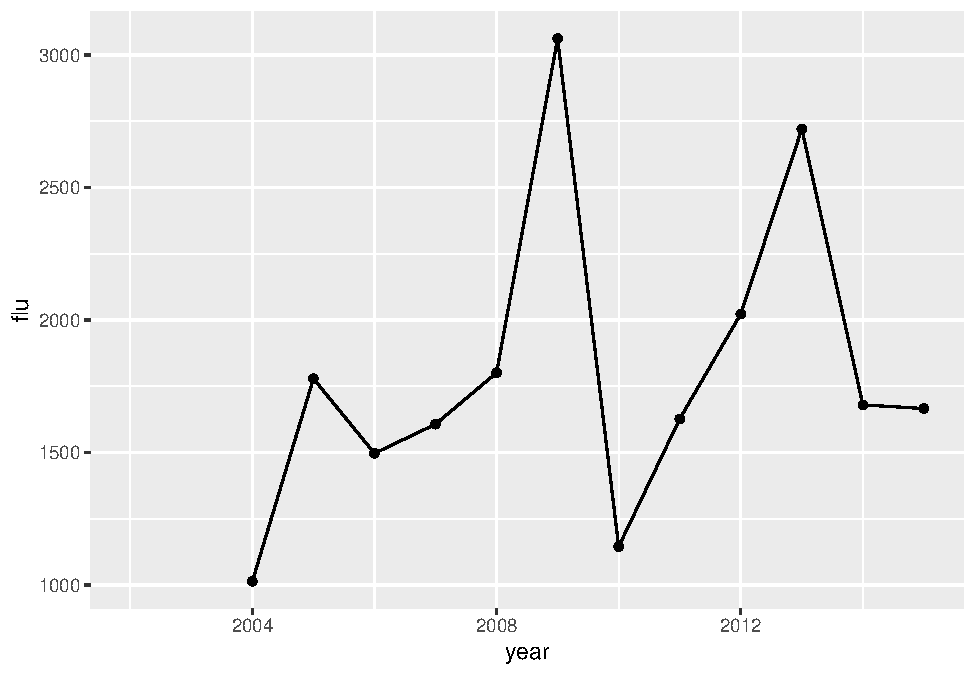
\includegraphics{Nexttry_files/figure-latex/unnamed-chunk-1-1.pdf}

\begin{Shaded}
\begin{Highlighting}[]
\NormalTok{alltogether }\SpecialCharTok{\%\textgreater{}\%} \FunctionTok{filter}\NormalTok{(country }\SpecialCharTok{==} \StringTok{"Argentina"}\NormalTok{) }\SpecialCharTok{\%\textgreater{}\%}
  \FunctionTok{ggplot}\NormalTok{() }\SpecialCharTok{+} 
  \FunctionTok{geom\_line}\NormalTok{(}\FunctionTok{aes}\NormalTok{(}\AttributeTok{y =}\NormalTok{ dengue,}\AttributeTok{x=}\NormalTok{year, }\AttributeTok{colour =} \StringTok{"green"}\NormalTok{),) }\SpecialCharTok{+} 
  \FunctionTok{geom\_line}\NormalTok{(}\FunctionTok{aes}\NormalTok{(}\AttributeTok{y =}\NormalTok{ flu,}\AttributeTok{x=}\NormalTok{year, }\AttributeTok{colour =} \StringTok{"red"}\NormalTok{))}
\end{Highlighting}
\end{Shaded}

\begin{verbatim}
## Warning: Removed 2 row(s) containing missing values (geom_path).
\end{verbatim}

\begin{verbatim}
## Warning: Removed 2 row(s) containing missing values (geom_path).
\end{verbatim}

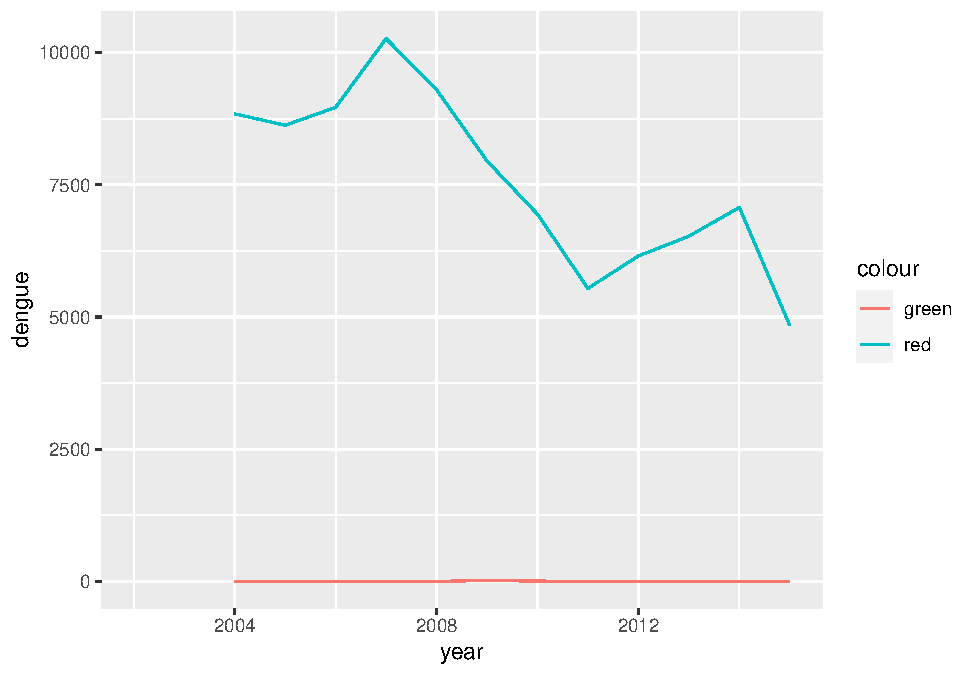
\includegraphics{Nexttry_files/figure-latex/unnamed-chunk-1-2.pdf}

\begin{Shaded}
\begin{Highlighting}[]
\FunctionTok{ggplot}\NormalTok{(}\AttributeTok{data =}\NormalTok{ alltogether, }\FunctionTok{aes}\NormalTok{(}\AttributeTok{x =}\NormalTok{ continent, }\AttributeTok{y =}\NormalTok{ flu)) }\SpecialCharTok{+}
  \FunctionTok{geom\_boxplot}\NormalTok{(}\FunctionTok{aes}\NormalTok{(}\AttributeTok{fill =}\NormalTok{ continent))}
\end{Highlighting}
\end{Shaded}

\begin{verbatim}
## Warning: Removed 72 rows containing non-finite values (stat_boxplot).
\end{verbatim}

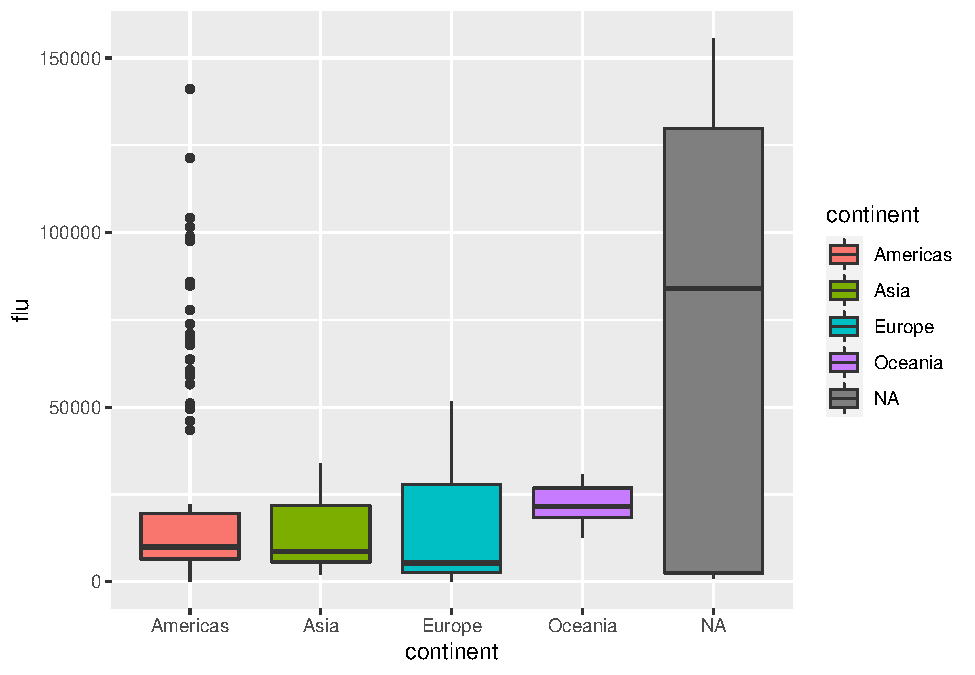
\includegraphics{Nexttry_files/figure-latex/unnamed-chunk-1-3.pdf}

\begin{Shaded}
\begin{Highlighting}[]
\FunctionTok{shapiro.test}\NormalTok{(alltogether}\SpecialCharTok{$}\NormalTok{fertility)}
\end{Highlighting}
\end{Shaded}

\begin{verbatim}
## 
##  Shapiro-Wilk normality test
## 
## data:  alltogether$fertility
## W = 0.84528, p-value < 2.2e-16
\end{verbatim}

\begin{Shaded}
\begin{Highlighting}[]
\FunctionTok{shapiro.test}\NormalTok{(alltogether}\SpecialCharTok{$}\NormalTok{flu)}
\end{Highlighting}
\end{Shaded}

\begin{verbatim}
## 
##  Shapiro-Wilk normality test
## 
## data:  alltogether$flu
## W = 0.70363, p-value < 2.2e-16
\end{verbatim}

\begin{Shaded}
\begin{Highlighting}[]
\FunctionTok{shapiro.test}\NormalTok{(alltogether}\SpecialCharTok{$}\NormalTok{dengue)}
\end{Highlighting}
\end{Shaded}

\begin{verbatim}
## 
##  Shapiro-Wilk normality test
## 
## data:  alltogether$dengue
## W = 0.91218, p-value = 0.0009743
\end{verbatim}

\begin{Shaded}
\begin{Highlighting}[]
\FunctionTok{shapiro.test}\NormalTok{(alltogether}\SpecialCharTok{$}\NormalTok{infant\_mortality)}
\end{Highlighting}
\end{Shaded}

\begin{verbatim}
## 
##  Shapiro-Wilk normality test
## 
## data:  alltogether$infant_mortality
## W = 0.75988, p-value < 2.2e-16
\end{verbatim}

\begin{Shaded}
\begin{Highlighting}[]
\FunctionTok{shapiro.test}\NormalTok{(alltogether}\SpecialCharTok{$}\NormalTok{life\_expectancy)}
\end{Highlighting}
\end{Shaded}

\begin{verbatim}
## 
##  Shapiro-Wilk normality test
## 
## data:  alltogether$life_expectancy
## W = 0.93264, p-value = 9.214e-12
\end{verbatim}

\begin{Shaded}
\begin{Highlighting}[]
\FunctionTok{shapiro.test}\NormalTok{(alltogether}\SpecialCharTok{$}\NormalTok{gdp)}
\end{Highlighting}
\end{Shaded}

\begin{verbatim}
## 
##  Shapiro-Wilk normality test
## 
## data:  alltogether$gdp
## W = 0.53327, p-value < 2.2e-16
\end{verbatim}

\begin{Shaded}
\begin{Highlighting}[]
\FunctionTok{shapiro.test}\NormalTok{(alltogether}\SpecialCharTok{$}\NormalTok{population)}
\end{Highlighting}
\end{Shaded}

\begin{verbatim}
## 
##  Shapiro-Wilk normality test
## 
## data:  alltogether$population
## W = 0.74646, p-value < 2.2e-16
\end{verbatim}

\hypertarget{my-own-package}{%
\chapter{My own package}\label{my-own-package}}

\hypertarget{parameters}{%
\chapter{Parameters}\label{parameters}}

\hypertarget{looking-ahead}{%
\chapter{Looking ahead}\label{looking-ahead}}

\hypertarget{appendix}{%
\chapter{Appendix}\label{appendix}}

\textbf{This code belongs to chapter 3}
I dont let this script run because then I get a error because of the plots are to large

R code for:
L?pez Steinmetz L.C., Dutto Florio M.A., Leyes C.A., Fong S.B., Rigalli A. \& Godoy J.C.
Levels and predictors of depression, anxiety, and suicidal risk during COVID-19 pandemic in Argentina: The impacts of quarantine extensions on mental health state.
\#```\{r\}

library(tidyverse)
library(readxl)\\
\# Load the dataset:
table\textless-read\_excel(``data/Peer/dataset.xlsx'')
summary(table)

\hypertarget{sub-title-methods-sample-and-procedure}{%
\subparagraph{SUB-TITLE: METHODS \textgreater{} Sample and procedure}\label{sub-title-methods-sample-and-procedure}}

\hypertarget{sample-n-1100}{%
\chapter{SAMPLE N = 1100}\label{sample-n-1100}}

\hypertarget{distribution-by-sex}{%
\chapter{Distribution by sex:}\label{distribution-by-sex}}

table(table\(SEX) # Absolute frequencies: Men = 217, Women = 883 prop.table(table(table\)SEX))*100
\# Percentages: Men = 19.72727\%, Women = 80.27273\%

\hypertarget{central-tendency-measures-by-age-entire-sample}{%
\chapter{Central tendency measures by age (entire sample)}\label{central-tendency-measures-by-age-entire-sample}}

\hypertarget{mean}{%
\chapter{Mean}\label{mean}}

mean(table\$AGE)
\# Age: mean = 31.45273

\hypertarget{standard-deviation-sd}{%
\chapter{Standard deviation (sd)}\label{standard-deviation-sd}}

sd(table\$AGE)
\# Age: sd = 11.7824

\hypertarget{standard-error-sem}{%
\chapter{Standard error (sem)}\label{standard-error-sem}}

library(``plotrix'')
std.error(table\$AGE)
\# Age: sem = 0.3552526

\hypertarget{median}{%
\chapter{median}\label{median}}

median(table\$AGE)
\# Age: median = 28

\hypertarget{sub-title-methods-data-analysis}{%
\subparagraph{SUB-TITLE: METHODS \textgreater{} Data analysis}\label{sub-title-methods-data-analysis}}

\hypertarget{to-test-skewness-and-kurtosis-criteria-range-of-acceptable-values-or-near-to--3-and-3-brown-2006.}{%
\chapter{To test Skewness and Kurtosis \# Criteria: range of acceptable values or near to -3 and +3 (Brown, 2006).}\label{to-test-skewness-and-kurtosis-criteria-range-of-acceptable-values-or-near-to--3-and-3-brown-2006.}}

\hypertarget{reference-brown-t.-a.-2006.-confirmatory-factor-analysis-for-applied-research.-new-york-guilford-press.}{%
\chapter{Reference: Brown, T. A. (2006). Confirmatory factor analysis for applied research. New York: Guilford Press.}\label{reference-brown-t.-a.-2006.-confirmatory-factor-analysis-for-applied-research.-new-york-guilford-press.}}

library(moments)

\hypertarget{depression}{%
\chapter{DEPRESSION}\label{depression}}

skewness(table\(DEPRESSION) # skewness DEPRESSION = 1.014193 kurtosis(table\)DEPRESSION)
\# kurtosis DEPRESSION = 3.789272

table \textless- rename(table, ``ANXIETY\_STATE'' = ``ANXIETY STATE'',
``ANXIETY\_TRAIT'' = ``ANXIETY TRAIT'',
``SUIC\_RISK'' = ``SUIC RISK'',
``SUB\_PERIODS'' = ``SUB PERIODS'',
``MENTAL\_DISORDER\_HISTORY'' = ``MENTAL DISORDER HISTORY'',
``SUIC\_ATTEMPT\_HISTORY'' = ``SUIC ATTEMPT HISTORY'',
``LIVING\_WITH\_SOMEBODY'' = ``LIVING WITH SOMEBODY'',
``ECONOMIC\_INCOME'' = ``ECONOMIC INCOME'')
\# ANXIETY STATE
skewness(table\(ANXIETY_STATE) # skewness ANXIETY STATE = 0.2010007 kurtosis(table\)ANXIETY\_STATE)
\# kurtosis ANXIETY STATE = 2.341017

\hypertarget{anxiety-trait}{%
\chapter{ANXIETY TRAIT}\label{anxiety-trait}}

skewness(table\(ANXIETY_TRAIT) # skewness ANXIETY TRAIT = 0.2401163 kurtosis(table\)ANXIETY\_TRAIT)
\# kurtosis ANXIETY TRAIT = 2.354038

\hypertarget{suicidal-risk}{%
\chapter{SUICIDAL RISK}\label{suicidal-risk}}

skewness(table\(SUIC_RISK) # skewness SUICIDAL RISK = 0.8331517 kurtosis(table\)SUIC\_RISK)
\# kurtosis SUICIDAL RISK = 3.193105

\hypertarget{for-addresing-the-first-aim-we-divided-the-entire-sample-into-three-groups}{%
\chapter{For addresing the first aim, we divided the entire sample into three groups:}\label{for-addresing-the-first-aim-we-divided-the-entire-sample-into-three-groups}}

table(table\$SUB\_PERIODS)
\# first quarantine extension (1. EXT POST) = 362
\# second and third quarantine extensions (2. EXT POST) = 239
\# fourth quarantine extension (3. EXT POST) = 499

RESULTS

AIM 1

\hypertarget{load-this-library-for-computing-effect-sizes}{%
\chapter{Load this library for computing effect sizes:}\label{load-this-library-for-computing-effect-sizes}}

library(sjstats)

\hypertarget{differences-in-specific-mental-health-state-indicators-by-three-sub-periods-of-quarantine}{%
\subsection{Differences in specific mental health state indicators by three sub-periods of quarantine}\label{differences-in-specific-mental-health-state-indicators-by-three-sub-periods-of-quarantine}}

\hypertarget{ext-post-first-quarantine-extension}{%
\chapter{1. EXT POST = first quarantine extension}\label{ext-post-first-quarantine-extension}}

\hypertarget{ext-post-secondthird-quarantine-extensions}{%
\chapter{2./3. EXT POST = second/third quarantine extensions}\label{ext-post-secondthird-quarantine-extensions}}

\hypertarget{ext-post-fourth-quarantine-extension}{%
\chapter{4. EXT POST = fourth quarantine extension}\label{ext-post-fourth-quarantine-extension}}

\hypertarget{depression-1}{%
\chapter{DEPRESSION}\label{depression-1}}

anovatempdepr \textless- aov(table\(DEPRESSION~table\)SUB\_PERIODS)
anovatempdepr
summary(anovatempdepr)
plot(anovatempdepr)
pairwise.t.test(x = table\(DEPRESSION, g = table\)SUB\_PERIODS, p.adjust.method = ``bonferroni'', pool.sd = TRUE, paired = FALSE, alternative = ``two.sided'')

\hypertarget{significant-differences}{%
\chapter{significant differences}\label{significant-differences}}

\hypertarget{ext-post-1.-ext-post-p-adj-0.018}{%
\chapter{2./3. EXT POST-1. EXT POST p adj 0.018}\label{ext-post-1.-ext-post-p-adj-0.018}}

\hypertarget{ext-post-1.-ext-post-p-adj-1.3e-05}{%
\chapter{4. EXT POST-1. EXT POST p adj 1.3e-05}\label{ext-post-1.-ext-post-p-adj-1.3e-05}}

\#effectsize::cohens\_f(anovatempdepr, ci = 0.95, partial = TRUE, type = 1)

tapply(table\(DEPRESSION,factor(table\)SUB\_PERIODS),mean)
tapply(table\(DEPRESSION,factor(table\)SUB\_PERIODS),std.error)

library(gplots)
\# Figure S1 (Supplementary material)
plotmeans(table\(DEPRESSION~table\)SUB\_PERIODS, main=``Fig. S1. Depression by quarantine sub-periods. Mean plot with 95\% Confidence Interval'', cex.main = 0.8, ylab = ``Depression'', xlab = ``Quarantine's sub periods'')

mean(table\(DEPRESSION) # mean = 15.69545 std.error(table\)DEPRESSION) \# std. error = 0.3347087
\# Percentage distribution by cutoff score:
\# non clinically depressed:
prop.table(table(table\(DEPRESSION<20,table\)SUB\_PERIODS))\emph{100
\# clinically depressed:
prop.table(table(table\(DEPRESSION>=20,table\)SUB\_PERIODS))}100

\hypertarget{anxiety-state}{%
\chapter{ANXIETY STATE}\label{anxiety-state}}

anovatempanxstate \textless- aov(table\(ANXIETY_STATE~table\)SUB\_PERIODS)
anovatempanxstate
summary(anovatempanxstate)
plot(anovatempanxstate)
pairwise.t.test(x = table\(ANXIETY_STATE, g = table\)SUB\_PERIODS, p.adjust.method = ``bonferroni'', pool.sd = TRUE, paired = FALSE, alternative = ``two.sided'')
\# significant differences
\# 2./3. EXT POST-1. EXT POST p adj 0.0057
\# 4. EXT POST-1. EXT POST p adj 0.0038
\#effectsize::cohens\_f(anovatempanxstate, ci = 0.95, partial = TRUE, type = 1)

tapply(table\(ANXIETY_STATE,factor(table\)SUB\_PERIODS),mean)
tapply(table\(ANXIETY_STATE,factor(table\)SUB\_PERIODS),std.error)

\hypertarget{figure-s2-supplementary-material}{%
\chapter{Figure S2 (Supplementary material)}\label{figure-s2-supplementary-material}}

plotmeans(table\(ANXIETY_STATE~table\)SUB\_PERIODS, main=``Fig. S2. State-Anxiety by quarantine sub-periods. Mean plot with 95\% Confidence Interval'', cex.main = 0.8, ylab = ``State-Anxiety'', xlab = ``Quarantine's sub periods'')

mean(table\(ANXIETY_STATE) # mean = 31.77545 std.error(table\)ANXIETY\_STATE) \# std. error = 0.436393
\# low:
prop.table(table(table\(ANXIETY_STATE<32,table\)SUB\_PERIODS))\emph{100
\# high:
prop.table(table(table\(ANXIETY_STATE>=32,table\)SUB\_PERIODS))}100

\hypertarget{anxiety-trait-1}{%
\chapter{ANXIETY TRAIT}\label{anxiety-trait-1}}

anovatempanxtrait \textless- aov(table\(ANXIETY_TRAIT~table\)SUB\_PERIODS)
anovatempanxtrait
summary(anovatempanxtrait)
plot(anovatempanxtrait)
pairwise.t.test(x = table\(ANXIETY_TRAIT, g = table\)SUB\_PERIODS, p.adjust.method = ``bonferroni'', pool.sd = TRUE, paired = FALSE, alternative = ``two.sided'')
\# significant differences
\# 2./3. EXT POST-1. EXT POST p adj 0.046
\# 4. EXT POST-1. EXT POST p adj 0.022
\#effectsize::cohens\_f(anovatempanxtrait, ci = 0.95, partial = TRUE, type = 1)

tapply(table\(ANXIETY_TRAIT,factor(table\)SUB\_PERIODS),mean)
tapply(table\(ANXIETY_TRAIT,factor(table\)SUB\_PERIODS),std.error)

\hypertarget{figure-s3-supplementary-material}{%
\chapter{Figure S3 (Supplementary material)}\label{figure-s3-supplementary-material}}

plotmeans(table\(ANXIETY_TRAIT~table\)SUB\_PERIODS, main=``Fig. S3. Trait-Anxiety by quarantine sub-periods. Mean plot with 95\% Confidence Interval'', cex.main = 0.8, ylab = ``Trait-Anxiety'', xlab = ``Quarantine's sub periods'')

mean(table\(ANXIETY_TRAIT) # mean = 26.89727 std.error(table\)ANXIETY\_TRAIT) \# std. error = 0.3662711
\# low:
prop.table(table(table\(ANXIETY_TRAIT<27,table\)SUB\_PERIODS))\emph{100
\# high:
prop.table(table(table\(ANXIETY_TRAIT>=27,table\)SUB\_PERIODS))}100

\hypertarget{suicidal-risk-1}{%
\chapter{SUICIDAL RISK}\label{suicidal-risk-1}}

anovatempsuic \textless- aov(table\(SUIC_RISK~table\)SUB\_PERIODS)
anovatempsuic
summary(anovatempsuic)
plot(anovatempsuic)
pairwise.t.test(x = table\(SUIC_RISK, g = table\)SUB\_PERIODS, p.adjust.method = ``bonferroni'', pool.sd = TRUE, paired = FALSE, alternative = ``two.sided'')
\# significant differences
\# 4. EXT POST-1. EXT POST p adj 0.030
\#effectsize::cohens\_f(anovatempsuic, ci = 0.95, partial = TRUE, type = 1)

tapply(table\(SUIC_RISK,factor(table\)SUB\_PERIODS),mean)
tapply(table\(SUIC_RISK,factor(table\)SUB\_PERIODS),std.error)

\hypertarget{figure-s4-supplementary-material}{%
\chapter{Figure S4 (Supplementary material)}\label{figure-s4-supplementary-material}}

plotmeans(table\(SUIC_RISK~table\)SUB\_PERIODS, main=``Fig. S4. Suicidal risk by quarantine sub-periods. Mean plot with 95\% Confidence Interval'', cex.main = 0.8, ylab = ``Suicidal risk'', xlab = ``Quarantine's sub periods'')

mean(table\(SUIC_RISK) # mean = 30.32182 std.error(table\)SUIC\_RISK) \# std. error = 0.4926946
\# Percentage distribution by cutoff score:
\# low:
prop.table(table(table\(SUIC_RISK<30,table\)SUB\_PERIODS))\emph{100
\# moderate:
prop.table(table(table\(SUIC_RISK>=30&table\)SUIC\_RISK\textless=44,table\(SUB_PERIODS))*100 # high: prop.table(table(table\)SUIC\_RISK\textgreater=45,table\$SUB\_PERIODS))}100

AIM 2

\hypertarget{multiple-linear-regressions}{%
\section{2) Multiple linear regressions:}\label{multiple-linear-regressions}}

\hypertarget{we-performed-stepwise-selection-direction-both-using-the-stepaic-function-from-the-mass-package.}{%
\chapter{We performed stepwise selection (direction = both) using the stepAIC() function from the MASS package.}\label{we-performed-stepwise-selection-direction-both-using-the-stepaic-function-from-the-mass-package.}}

library(MASS)
\# stepAIC() performs stepwise model selection by exact AIC

\hypertarget{depression-2}{%
\subsubsection{DEPRESSION:}\label{depression-2}}

\hypertarget{stepwise-regression}{%
\chapter{Stepwise Regression}\label{stepwise-regression}}

fitwith\textless-lm(DEPRESSION\textasciitilde SEX+AGE+PROVINCE+EDUCATION+ECONOMIC\_INCOME+LIVING\_WITH\_SOMEBODY+MENTAL\_DISORDER\_HISTORY+SUIC\_ATTEMPT\_HISTORY+SUB\_PERIODS,data=table)
stepwith \textless- stepAIC(fitwith, trace=TRUE,direction=``both'')
stepwith
stepwith\$anova \# display results
\# Stepwise Model Path
\# Analysis of Deviance Table
\# Initial Model: DEPRESSION \textasciitilde{} SEX + AGE + PROVINCE + EDUCATION + ECONOMIC\_INCOME + LIVING\_WITH\_SOMEBODY + MENTAL\_DISORDER\_HISTORY + SUIC\_ATTEMPT\_HISTORY + SUB\_PERIODS
\# Start: AIC = 4951.51
\# Final Model: DEPRESSION \textasciitilde{} SEX + AGE + ECONOMIC\_INCOME + MENTAL\_DISORDER\_HISTORY + SUIC\_ATTEMPT\_HISTORY + SUB\_PERIODS
\# Stepwith: AIC = 4938.7
summary(stepwith)

\hypertarget{confidence-interval-of-best-fitted-model}{%
\chapter{95\% Confidence interval of best-fitted model:}\label{confidence-interval-of-best-fitted-model}}

confint(stepwith)

\hypertarget{error-rate-of-best-fitted-model}{%
\chapter{ERROR RATE of best-fitted model:}\label{error-rate-of-best-fitted-model}}

sigma(stepwith)/mean(table\$DEPRESSION)
\# 0.5989474
\# In our multiple regression example, the Residual Standard Error (RSE) or sigma is 9.401 corresponding to 60\% error rate.

par(mfrow=c(2,2))
\# Figure S5 (Supplementary material)
plot(stepwith)
par(mfrow=c(1,1))

\hypertarget{table-1}{%
\chapter{TABLE 1:}\label{table-1}}

\hypertarget{model-1-initial-model}{%
\chapter{Model 1: INITIAL MODEL:}\label{model-1-initial-model}}

model1\textless-lm(DEPRESSION\textasciitilde SEX+AGE+PROVINCE+EDUCATION+ECONOMIC\_INCOME+LIVING\_WITH\_SOMEBODY+MENTAL\_DISORDER\_HISTORY+SUIC\_ATTEMPT\_HISTORY+SUB\_PERIODS,data=table)
summary(model1)
\# YES significative p-value \textless{} 2.2e-16

\hypertarget{model-2-eliminates-province}{%
\chapter{Model 2 eliminates PROVINCE:}\label{model-2-eliminates-province}}

model2\textless-lm(DEPRESSION\textasciitilde SEX+AGE+EDUCATION+ECONOMIC\_INCOME+LIVING\_WITH\_SOMEBODY+MENTAL\_DISORDER\_HISTORY+SUIC\_ATTEMPT\_HISTORY+SUB\_PERIODS,data=table)
summary(model2)
\# YES significative p-value \textless{} 2.2e-16

\hypertarget{model-3-eliminates-education}{%
\chapter{Model 3 eliminates EDUCATION:}\label{model-3-eliminates-education}}

model3\textless-lm(DEPRESSION\textasciitilde SEX+AGE+ECONOMIC\_INCOME+LIVING\_WITH\_SOMEBODY+MENTAL\_DISORDER\_HISTORY+SUIC\_ATTEMPT\_HISTORY+SUB\_PERIODS,data=table)
summary(model3)
\# YES significative p-value \textless{} 2.2e-16

\hypertarget{model-4-eliminates-living_with_somebody}{%
\chapter{Model 4 eliminates LIVING\_WITH\_SOMEBODY:}\label{model-4-eliminates-living_with_somebody}}

model4\textless-lm(DEPRESSION\textasciitilde SEX+AGE+ECONOMIC\_INCOME+MENTAL\_DISORDER\_HISTORY+SUIC\_ATTEMPT\_HISTORY+SUB\_PERIODS,data=table)
summary(model4)
\# YES significative p-value \textless{} 2.2e-16

\hypertarget{considering-the-predictors-included-in-the-best-fitted-model-i.e.-stepwith-in-this-group-we-analyzed-the-smallest-possible-linear-model-for-each-specific-mhs-indicator-by-means-of-all-two-predictor-combinations.}{%
\section{Considering the predictors included in the best-fitted model (i.e., stepwith) in this group, we analyzed the smallest possible linear model for each specific MHS indicator by means of all two-predictor combinations.}\label{considering-the-predictors-included-in-the-best-fitted-model-i.e.-stepwith-in-this-group-we-analyzed-the-smallest-possible-linear-model-for-each-specific-mhs-indicator-by-means-of-all-two-predictor-combinations.}}

\hypertarget{we-performed-all-subsets-regression-using-the-regsubsets-function-from-the-leaps-package.}{%
\chapter{We performed all-subsets regression using the regsubsets() function from the leaps package.}\label{we-performed-all-subsets-regression-using-the-regsubsets-function-from-the-leaps-package.}}

\hypertarget{we-analyzed-the-three-best-models-for-two-predictor-subset-sizes.}{%
\chapter{We analyzed the three best models for two-predictor subset sizes.}\label{we-analyzed-the-three-best-models-for-two-predictor-subset-sizes.}}

library(leaps)
leapsbestwith\textless-regsubsets(DEPRESSION\textasciitilde SEX+AGE+ECONOMIC\_INCOME+MENTAL\_DISORDER\_HISTORY+SUIC\_ATTEMPT\_HISTORY+SUB\_PERIODS,data=table,nbest=3)
summary(leapsbestwith)
\# The best two-predictors model was: DEPRESSION \textasciitilde{} AGE + SUIC\_ATTEMPT\_HISTORY==no

plot(leapsbestwith,scale=``r2'')
plot(leapsbestwith,scale=``adjr2'')

\hypertarget{first-age-suic_attempt_history-no}{%
\chapter{First: AGE + SUIC\_ATTEMPT\_HISTORY (no):}\label{first-age-suic_attempt_history-no}}

besttwowithfirst\textless-lm(DEPRESSION\textasciitilde AGE+SUIC\_ATTEMPT\_HISTORY,data=table)
besttwowithfirst
summary(besttwowithfirst)
confint(besttwowithfirst)

\hypertarget{second-sex-woman-suic_attempt_history-no}{%
\chapter{Second: SEX (woman) + SUIC\_ATTEMPT\_HISTORY (no):}\label{second-sex-woman-suic_attempt_history-no}}

besttwowithsecond\textless-lm(DEPRESSION\textasciitilde SEX+SUIC\_ATTEMPT\_HISTORY,data=table)
besttwowithsecond
summary(besttwowithsecond)
confint(besttwowithsecond)

\hypertarget{third-suic_attempt_history-no-sub-periods-4.-ext-post}{%
\chapter{Third: SUIC\_ATTEMPT\_HISTORY (no) + SUB PERIODS (4. EXT POST):}\label{third-suic_attempt_history-no-sub-periods-4.-ext-post}}

besttwowiththird\textless-lm(DEPRESSION\textasciitilde SUIC\_ATTEMPT\_HISTORY+SUB\_PERIODS,data=table)
besttwowiththird
summary(besttwowiththird)
confint(besttwowiththird)

\hypertarget{anxiety-state-1}{%
\subsubsection{ANXIETY-STATE:}\label{anxiety-state-1}}

\hypertarget{stepwise-regression-1}{%
\chapter{Stepwise Regression}\label{stepwise-regression-1}}

fitwith\textless-lm(ANXIETY\_STATE\textasciitilde SEX+AGE+PROVINCE+EDUCATION+ECONOMIC\_INCOME+LIVING\_WITH\_SOMEBODY+MENTAL\_DISORDER\_HISTORY+SUIC\_ATTEMPT\_HISTORY+SUB\_PERIODS,data=table)
stepwith \textless- stepAIC(fitwith, trace=TRUE,direction=``both'')
stepwith
stepwith\$anova \# display results
\# Stepwise Model Path
\# Analysis of Deviance Table
\# Initial Model: ANXIETY\_STATE \textasciitilde{} SEX + AGE + PROVINCE + EDUCATION + ECONOMIC\_INCOME + LIVING\_WITH\_SOMEBODY + MENTAL\_DISORDER\_HISTORY + SUIC\_ATTEMPT\_HISTORY + SUB\_PERIODS
\# Start: AIC = 5679.05
\# Final Model: ANXIETY\_STATE \textasciitilde{} SEX + AGE + MENTAL\_DISORDER\_HISTORY + SUIC\_ATTEMPT\_HISTORY + SUB\_PERIODS
\# Stepwith: AIC = 5660.25
summary(stepwith)

\hypertarget{confidence-interval-of-best-fitted-model-1}{%
\chapter{95\% Confidence interval of best-fitted model:}\label{confidence-interval-of-best-fitted-model-1}}

confint(stepwith)

\hypertarget{error-rate-of-best-fitted-model-1}{%
\chapter{ERROR RATE of best-fitted model:}\label{error-rate-of-best-fitted-model-1}}

sigma(stepwith)/mean(table\$ANXIETY\_STATE)
\# 0.4108702
\# In our multiple regression example, the Residual Standard Error (RSE) or sigma is 13.06 corresponding to 41\% error rate.

par(mfrow=c(2,2))
\# Figure S6 (Supplementary material)
plot(stepwith)
par(mfrow=c(1,1))

\hypertarget{table-1-1}{%
\chapter{TABLE 1:}\label{table-1-1}}

\hypertarget{model-1-initial-model-1}{%
\chapter{Model 1: INITIAL MODEL:}\label{model-1-initial-model-1}}

model1\textless-lm(ANXIETY\_STATE\textasciitilde SEX+AGE+PROVINCE+EDUCATION+ECONOMIC\_INCOME+LIVING\_WITH\_SOMEBODY+MENTAL\_DISORDER\_HISTORY+SUIC\_ATTEMPT\_HISTORY+SUB\_PERIODS,data=table)
summary(model1)
\# YES significative p-value \textless{} 2.2e-16

\hypertarget{model-2-eliminates-province-1}{%
\chapter{Model 2 eliminates PROVINCE:}\label{model-2-eliminates-province-1}}

model2\textless-lm(ANXIETY\_STATE\textasciitilde SEX+AGE+EDUCATION+ECONOMIC\_INCOME+LIVING\_WITH\_SOMEBODY+MENTAL\_DISORDER\_HISTORY+SUIC\_ATTEMPT\_HISTORY+SUB\_PERIODS,data=table)
summary(model2)
\# YES significative p-value \textless{} 2.2e-16

\hypertarget{model-3-eliminates-education-1}{%
\chapter{Model 3 eliminates EDUCATION:}\label{model-3-eliminates-education-1}}

model3\textless-lm(ANXIETY\_STATE\textasciitilde SEX+AGE+ECONOMIC\_INCOME+LIVING\_WITH\_SOMEBODY+MENTAL\_DISORDER\_HISTORY+SUIC\_ATTEMPT\_HISTORY+SUB\_PERIODS,data=table)
summary(model3)
\# YES significative p-value \textless{} 2.2e-16

\hypertarget{model-4-eliminates-economic_income}{%
\chapter{Model 4 eliminates ECONOMIC\_INCOME:}\label{model-4-eliminates-economic_income}}

model4\textless-lm(ANXIETY\_STATE\textasciitilde SEX+AGE+LIVING\_WITH\_SOMEBODY+MENTAL\_DISORDER\_HISTORY+SUIC\_ATTEMPT\_HISTORY+SUB\_PERIODS,data=table)
summary(model4)
\# YES significative p-value \textless{} 2.2e-16

\hypertarget{model-5-eliminates-living_with_somebody}{%
\chapter{Model 5 eliminates LIVING\_WITH\_SOMEBODY:}\label{model-5-eliminates-living_with_somebody}}

model5\textless-lm(ANXIETY\_STATE\textasciitilde SEX+AGE+MENTAL\_DISORDER\_HISTORY+SUIC\_ATTEMPT\_HISTORY+SUB\_PERIODS,data=table)
summary(model5)
\# YES significative p-value \textless{} 2.2e-16

\hypertarget{considering-the-predictors-included-in-the-best-fitted-model-i.e.-stepwith-in-this-group-we-analyzed-the-smallest-possible-linear-model-for-each-specific-mhs-indicator-by-means-of-all-two-predictor-combinations.-1}{%
\section{Considering the predictors included in the best-fitted model (i.e., stepwith) in this group, we analyzed the smallest possible linear model for each specific MHS indicator by means of all two-predictor combinations.}\label{considering-the-predictors-included-in-the-best-fitted-model-i.e.-stepwith-in-this-group-we-analyzed-the-smallest-possible-linear-model-for-each-specific-mhs-indicator-by-means-of-all-two-predictor-combinations.-1}}

\hypertarget{we-performed-all-subsets-regression-using-the-regsubsets-function-from-the-leaps-package.-1}{%
\chapter{We performed all-subsets regression using the regsubsets() function from the leaps package.}\label{we-performed-all-subsets-regression-using-the-regsubsets-function-from-the-leaps-package.-1}}

\hypertarget{we-analyzed-the-three-best-models-for-two-predictor-subset-sizes.-1}{%
\chapter{We analyzed the three best models for two-predictor subset sizes.}\label{we-analyzed-the-three-best-models-for-two-predictor-subset-sizes.-1}}

leapsbestwith\textless-regsubsets(ANXIETY\_STATE\textasciitilde SEX+AGE+MENTAL\_DISORDER\_HISTORY+SUIC\_ATTEMPT\_HISTORY+SUB\_PERIODS,data=table,nbest=3)
summary(leapsbestwith)
\# The best two-predictors model was: ANXIETY\_STATE \textasciitilde{} AGE + SUIC\_ATTEMPT\_HISTORY==no

plot(leapsbestwith,scale=``r2'')
plot(leapsbestwith,scale=``adjr2'')

\hypertarget{first-age-suic_attempt_history-no-1}{%
\chapter{First: AGE + SUIC\_ATTEMPT\_HISTORY (no):}\label{first-age-suic_attempt_history-no-1}}

besttwowithfirst\textless-lm(ANXIETY\_STATE\textasciitilde AGE+SUIC\_ATTEMPT\_HISTORY,data=table)
besttwowithfirst
summary(besttwowithfirst)
confint(besttwowithfirst)

\hypertarget{second-mental-disorder-yes-suic_attempt_history-no}{%
\chapter{Second: MENTAL DISORDER (yes) + SUIC\_ATTEMPT\_HISTORY (no):}\label{second-mental-disorder-yes-suic_attempt_history-no}}

besttwowithsecond\textless-lm(ANXIETY\_STATE\textasciitilde MENTAL\_DISORDER\_HISTORY+SUIC\_ATTEMPT\_HISTORY,data=table)
besttwowithsecond
summary(besttwowithsecond)
confint(besttwowithsecond)

\hypertarget{third-age-mental-disorder-yes}{%
\chapter{Third: AGE + MENTAL DISORDER (yes):}\label{third-age-mental-disorder-yes}}

besttwowiththird\textless-lm(ANXIETY\_STATE\textasciitilde AGE+MENTAL\_DISORDER\_HISTORY,data=table)
besttwowiththird
summary(besttwowiththird)
confint(besttwowiththird)

\hypertarget{anxiety-trait-2}{%
\subsubsection{ANXIETY-TRAIT:}\label{anxiety-trait-2}}

\hypertarget{stepwise-regression-2}{%
\chapter{Stepwise Regression}\label{stepwise-regression-2}}

fitwith\textless-lm(ANXIETY\_TRAIT\textasciitilde SEX+AGE+PROVINCE+EDUCATION+ECONOMIC\_INCOME+LIVING\_WITH\_SOMEBODY+MENTAL\_DISORDER\_HISTORY+SUIC\_ATTEMPT\_HISTORY+SUB\_PERIODS,data=table)
stepwith \textless- stepAIC(fitwith, trace=TRUE,direction=``both'')
stepwith
stepwith\$anova \# display results
\# Stepwise Model Path
\# Analysis of Deviance Table
\# Initial Model: ANXIETY\_TRAIT \textasciitilde{} SEX + AGE + PROVINCE + EDUCATION + ECONOMIC\_INCOME + LIVING\_WITH\_SOMEBODY + MENTAL\_DISORDER\_HISTORY + SUIC\_ATTEMPT\_HISTORY + SUB\_PERIODS
\# Start: AIC = 5137.82
\# Final Model: ANXIETY\_TRAIT \textasciitilde{} SEX + AGE + ECONOMIC\_INCOME + MENTAL\_DISORDER\_HISTORY + SUIC\_ATTEMPT\_HISTORY
\# Stepwith: AIC = 5123.92
summary(stepwith)

\hypertarget{confidence-interval-of-best-fitted-model-2}{%
\chapter{95\% Confidence interval of best-fitted model:}\label{confidence-interval-of-best-fitted-model-2}}

confint(stepwith)

\hypertarget{error-rate-of-best-fitted-model-2}{%
\chapter{ERROR RATE of best-fitted model:}\label{error-rate-of-best-fitted-model-2}}

sigma(stepwith)/mean(table\$ANXIETY\_TRAIT)
\# 0.380548
\# In our multiple regression example, the Residual Standard Error (RSE) or sigma is 10.24 corresponding to 38\% error rate.

par(mfrow=c(2,2))
\# Figure S7 (Supplementary material)
plot(stepwith)
par(mfrow=c(1,1))

\hypertarget{table-1-2}{%
\chapter{TABLE 1:}\label{table-1-2}}

\hypertarget{model-1-initial-model-2}{%
\chapter{Model 1: INITIAL MODEL:}\label{model-1-initial-model-2}}

model1\textless-lm(ANXIETY\_TRAIT\textasciitilde SEX+AGE+PROVINCE+EDUCATION+ECONOMIC\_INCOME+LIVING\_WITH\_SOMEBODY+MENTAL\_DISORDER\_HISTORY+SUIC\_ATTEMPT\_HISTORY+SUB\_PERIODS,data=table)
summary(model1)
\# YES significative p-value \textless{} 2.2e-16

\hypertarget{model-2-eliminates-education}{%
\chapter{Model 2 eliminates EDUCATION:}\label{model-2-eliminates-education}}

model2\textless-lm(ANXIETY\_TRAIT\textasciitilde SEX+AGE+PROVINCE+ECONOMIC\_INCOME+LIVING\_WITH\_SOMEBODY+MENTAL\_DISORDER\_HISTORY+SUIC\_ATTEMPT\_HISTORY+SUB\_PERIODS,data=table)
summary(model2)
\# YES significative p-value \textless{} 2.2e-16

\hypertarget{model-3-eliminates-province}{%
\chapter{Model 3 eliminates PROVINCE:}\label{model-3-eliminates-province}}

model3\textless-lm(ANXIETY\_TRAIT\textasciitilde SEX+AGE+ECONOMIC\_INCOME+LIVING\_WITH\_SOMEBODY+MENTAL\_DISORDER\_HISTORY+SUIC\_ATTEMPT\_HISTORY+SUB\_PERIODS,data=table)
summary(model3)
\# YES significative p-value \textless{} 2.2e-16

\hypertarget{model-4-eliminates-living_with_somebody-1}{%
\chapter{Model 4 eliminates LIVING\_WITH\_SOMEBODY:}\label{model-4-eliminates-living_with_somebody-1}}

model4\textless-lm(ANXIETY\_TRAIT\textasciitilde SEX+AGE+ECONOMIC\_INCOME+MENTAL\_DISORDER\_HISTORY+SUIC\_ATTEMPT\_HISTORY+SUB\_PERIODS,data=table)
summary(model4)
\# YES significative p-value \textless{} 2.2e-16

\hypertarget{model-5-eliminates-sub-periods}{%
\chapter{Model 5 eliminates SUB PERIODS:}\label{model-5-eliminates-sub-periods}}

model4\textless-lm(ANXIETY\_TRAIT\textasciitilde SEX+AGE+ECONOMIC\_INCOME+MENTAL\_DISORDER\_HISTORY+SUIC\_ATTEMPT\_HISTORY,data=table)
summary(model4)
\# YES significative p-value \textless{} 2.2e-16

\hypertarget{considering-the-predictors-included-in-the-best-fitted-model-i.e.-stepwith-in-this-group-we-analyzed-the-smallest-possible-linear-model-for-each-specific-mhs-indicator-by-means-of-all-two-predictor-combinations.-2}{%
\section{Considering the predictors included in the best-fitted model (i.e., stepwith) in this group, we analyzed the smallest possible linear model for each specific MHS indicator by means of all two-predictor combinations.}\label{considering-the-predictors-included-in-the-best-fitted-model-i.e.-stepwith-in-this-group-we-analyzed-the-smallest-possible-linear-model-for-each-specific-mhs-indicator-by-means-of-all-two-predictor-combinations.-2}}

\hypertarget{we-performed-all-subsets-regression-using-the-regsubsets-function-from-the-leaps-package.-2}{%
\chapter{We performed all-subsets regression using the regsubsets() function from the leaps package.}\label{we-performed-all-subsets-regression-using-the-regsubsets-function-from-the-leaps-package.-2}}

\hypertarget{we-analyzed-the-three-best-models-for-two-predictor-subset-sizes.-2}{%
\chapter{We analyzed the three best models for two-predictor subset sizes.}\label{we-analyzed-the-three-best-models-for-two-predictor-subset-sizes.-2}}

leapsbestwith\textless-regsubsets(ANXIETY\_TRAIT\textasciitilde SEX+AGE+ECONOMIC\_INCOME+MENTAL\_DISORDER\_HISTORY+SUIC\_ATTEMPT\_HISTORY,data=table,nbest=3)
summary(leapsbestwith)
\# The best two-predictors model was: ANXIETY\_STATE \textasciitilde{} AGE + SUIC\_ATTEMPT\_HISTORY==no

plot(leapsbestwith,scale=``r2'')
plot(leapsbestwith,scale=``adjr2'')

\hypertarget{first-age-suic_attempt_history-no-2}{%
\chapter{First: AGE + SUIC\_ATTEMPT\_HISTORY (no):}\label{first-age-suic_attempt_history-no-2}}

besttwowithfirst\textless-lm(ANXIETY\_TRAIT\textasciitilde AGE+SUIC\_ATTEMPT\_HISTORY,data=table)
besttwowithfirst
summary(besttwowithfirst)
confint(besttwowithfirst)

\hypertarget{second-mental-disorder-yes-suic_attempt_history-no-1}{%
\chapter{Second: MENTAL DISORDER (yes) + SUIC\_ATTEMPT\_HISTORY (no):}\label{second-mental-disorder-yes-suic_attempt_history-no-1}}

besttwowithsecond\textless-lm(ANXIETY\_TRAIT\textasciitilde MENTAL\_DISORDER\_HISTORY+SUIC\_ATTEMPT\_HISTORY,data=table)
besttwowithsecond
summary(besttwowithsecond)
confint(besttwowithsecond)

\hypertarget{third-sex-woman-suic_attempt_history-no}{%
\chapter{Third: SEX (woman) + SUIC\_ATTEMPT\_HISTORY (no):}\label{third-sex-woman-suic_attempt_history-no}}

besttwowiththird\textless-lm(ANXIETY\_TRAIT\textasciitilde SEX+SUIC\_ATTEMPT\_HISTORY,data=table)
besttwowiththird
summary(besttwowiththird)
confint(besttwowiththird)

\hypertarget{suicidal-risk-2}{%
\subsubsection{SUICIDAL RISK:}\label{suicidal-risk-2}}

\hypertarget{stepwise-regression-3}{%
\chapter{Stepwise Regression}\label{stepwise-regression-3}}

fitwith\textless-lm(SUIC\_RISK\textasciitilde SEX+AGE+PROVINCE+EDUCATION+ECONOMIC\_INCOME+LIVING\_WITH\_SOMEBODY+MENTAL\_DISORDER\_HISTORY+SUIC\_ATTEMPT\_HISTORY+SUB\_PERIODS,data=table)
stepwith \textless- stepAIC(fitwith, trace=TRUE,direction=``both'')
stepwith
stepwith\$anova \# display results
\# Stepwise Model Path
\# Analysis of Deviance Table
\# Initial Model: SUIC\_RISK \textasciitilde{} SEX + AGE + PROVINCE + EDUCATION + ECONOMIC\_INCOME + LIVING\_WITH\_SOMEBODY + MENTAL\_DISORDER\_HISTORY + SUIC\_ATTEMPT\_HISTORY + SUB\_PERIODS
\# Start: AIC = 5732.18
\# Final Model: SUIC\_RISK \textasciitilde{} SEX + AGE + ECONOMIC\_INCOME + MENTAL\_DISORDER\_HISTORY + SUIC\_ATTEMPT\_HISTORY
\# Stepwith: AIC = 5715.52
summary(stepwith)

\hypertarget{confidence-interval-of-best-fitted-model-3}{%
\chapter{95\% Confidence interval of best-fitted model:}\label{confidence-interval-of-best-fitted-model-3}}

confint(stepwith)

\hypertarget{error-rate-of-best-fitted-model-3}{%
\chapter{ERROR RATE of best-fitted model:}\label{error-rate-of-best-fitted-model-3}}

sigma(stepwith)/mean(table\$SUIC\_RISK)
\# 0.4417225
\# In our multiple regression example, the Residual Standard Error (RSE) or sigma is 13.39 corresponding to 44\% error rate.

par(mfrow=c(2,2))
\# Figure S8 (Supplementary material)
plot(stepwith)
par(mfrow=c(1,1))

\hypertarget{table-1-3}{%
\chapter{TABLE 1:}\label{table-1-3}}

\hypertarget{model-1-initial-model-3}{%
\chapter{Model 1: INITIAL MODEL:}\label{model-1-initial-model-3}}

model1\textless-lm(SUIC\_RISK\textasciitilde SEX+AGE+PROVINCE+EDUCATION+ECONOMIC\_INCOME+LIVING\_WITH\_SOMEBODY+MENTAL\_DISORDER\_HISTORY+SUIC\_ATTEMPT\_HISTORY+SUB\_PERIODS,data=table)
summary(model1)
\# YES significative p-value \textless{} 2.2e-16

\hypertarget{model-2-eliminates-province-2}{%
\chapter{Model 2 eliminates PROVINCE:}\label{model-2-eliminates-province-2}}

model2\textless-lm(SUIC\_RISK\textasciitilde SEX+AGE+EDUCATION+ECONOMIC\_INCOME+LIVING\_WITH\_SOMEBODY+MENTAL\_DISORDER\_HISTORY+SUIC\_ATTEMPT\_HISTORY+SUB\_PERIODS,data=table)
summary(model2)
\# YES significative p-value \textless{} 2.2e-16

\hypertarget{model-3-eliminates-education-2}{%
\chapter{Model 3 eliminates EDUCATION:}\label{model-3-eliminates-education-2}}

model3\textless-lm(SUIC\_RISK\textasciitilde SEX+AGE+ECONOMIC\_INCOME+LIVING\_WITH\_SOMEBODY+MENTAL\_DISORDER\_HISTORY+SUIC\_ATTEMPT\_HISTORY+SUB\_PERIODS,data=table)
summary(model3)
\# YES significative p-value \textless{} 2.2e-16

\hypertarget{model-4-eliminates-living_with_somebody-2}{%
\chapter{Model 4 eliminates LIVING\_WITH\_SOMEBODY:}\label{model-4-eliminates-living_with_somebody-2}}

model4\textless-lm(SUIC\_RISK\textasciitilde SEX+AGE+ECONOMIC\_INCOME+MENTAL\_DISORDER\_HISTORY+SUIC\_ATTEMPT\_HISTORY+SUB\_PERIODS,data=table)
summary(model4)
\# YES significative p-value \textless{} 2.2e-16

\hypertarget{model-5-eliminates-sub-periods-1}{%
\chapter{Model 5 eliminates SUB PERIODS:}\label{model-5-eliminates-sub-periods-1}}

model5\textless-lm(SUIC\_RISK\textasciitilde SEX+AGE+ECONOMIC\_INCOME+MENTAL\_DISORDER\_HISTORY+SUIC\_ATTEMPT\_HISTORY,data=table)
summary(model5)
\# YES significative p-value \textless{} 2.2e-16

\hypertarget{considering-the-predictors-included-in-the-best-fitted-model-i.e.-stepwith-in-this-group-we-analyzed-the-smallest-possible-linear-model-for-each-specific-mhs-indicator-by-means-of-all-two-predictor-combinations.-3}{%
\section{Considering the predictors included in the best-fitted model (i.e., stepwith) in this group, we analyzed the smallest possible linear model for each specific MHS indicator by means of all two-predictor combinations.}\label{considering-the-predictors-included-in-the-best-fitted-model-i.e.-stepwith-in-this-group-we-analyzed-the-smallest-possible-linear-model-for-each-specific-mhs-indicator-by-means-of-all-two-predictor-combinations.-3}}

\hypertarget{we-performed-all-subsets-regression-using-the-regsubsets-function-from-the-leaps-package.-3}{%
\chapter{We performed all-subsets regression using the regsubsets() function from the leaps package.}\label{we-performed-all-subsets-regression-using-the-regsubsets-function-from-the-leaps-package.-3}}

\hypertarget{we-analyzed-the-three-best-models-for-two-predictor-subset-sizes.-3}{%
\chapter{We analyzed the three best models for two-predictor subset sizes.}\label{we-analyzed-the-three-best-models-for-two-predictor-subset-sizes.-3}}

leapsbestwith\textless-regsubsets(SUIC\_RISK\textasciitilde SEX+AGE+ECONOMIC\_INCOME+MENTAL\_DISORDER\_HISTORY+SUIC\_ATTEMPT\_HISTORY,data=table,nbest=3)
summary(leapsbestwith)
\# The best two-predictors model was: ANXIETY\_STATE \textasciitilde{} AGE + SUIC\_ATTEMPT\_HISTORY==no

plot(leapsbestwith,scale=``r2'')
plot(leapsbestwith,scale=``adjr2'')

\hypertarget{first-age-suic_attempt_history-no-3}{%
\chapter{First: AGE + SUIC\_ATTEMPT\_HISTORY (no):}\label{first-age-suic_attempt_history-no-3}}

besttwowithfirst\textless-lm(SUIC\_RISK\textasciitilde AGE+SUIC\_ATTEMPT\_HISTORY,data=table)
besttwowithfirst
summary(besttwowithfirst)
confint(besttwowithfirst)

\hypertarget{second-mental-disorder-yes-suic_attempt_history-no-2}{%
\chapter{Second: MENTAL DISORDER (yes) + SUIC\_ATTEMPT\_HISTORY (no):}\label{second-mental-disorder-yes-suic_attempt_history-no-2}}

besttwowithsecond\textless-lm(SUIC\_RISK\textasciitilde MENTAL\_DISORDER\_HISTORY+SUIC\_ATTEMPT\_HISTORY,data=table)
besttwowithsecond
summary(besttwowithsecond)
confint(besttwowithsecond)

\hypertarget{third-economic_income-yes-suic_attempt_history-no}{%
\chapter{Third: ECONOMIC\_INCOME (yes) + SUIC\_ATTEMPT\_HISTORY (no):}\label{third-economic_income-yes-suic_attempt_history-no}}

besttwowiththird\textless-lm(SUIC\_RISK\textasciitilde ECONOMIC\_INCOME+SUIC\_ATTEMPT\_HISTORY,data=table)
besttwowiththird
summary(besttwowiththird)
confint(besttwowiththird)

\begin{verbatim}

\end{verbatim}

  \bibliography{book.bib,packages.bib,referenties.bib}

\end{document}
